\begin{frame}

\begin{center}
{\LARGE Escape Slides}
\end{center}

\end{frame}

%-------------------------------------------------------

%-------------------------------------------------------

\begin{frame}[label=bachmann]{Bachmann, Cabellero and Engel (2013)}

While reading papers for my own work, I found this nice statement in \href{https://www.aeaweb.org/articles?id=10.1257/mac.5.4.29}{Bachmann \textit{et al} (2013)}\ldots

\vspace{5mm}
\begin{quote}
Our calibration begins by noting that the objective in any dynamic macroeconomic model is to trace the impact of aggregate shocks on aggregate endogenous variables
\end{quote}

\end{frame}

%-------------------------------------------------------

%-------------------------------------------------------

\begin{frame}{Bachmann, Cabellero and Engel (2013)}

This reflects the standard attitude in modern macro
\begin{itemize}
\item	The state typically will not only involve exogenous shocks
\item	The state may involve accumulated capital (or complicated objects like the distribution of wealth over households) that themselves are endogenous, but predetermined in $t$
\item	But we typically talk about economies responding to `innovations' or `impulses' to the shock process
\item	These innovations are - in the context of the model - the only true `source' of curve shifts
\item	If you know how \textit{all} the `curves' shift, then you can calculate fluctuations in the endogenous variable in equilibrium
\end{itemize}

\end{frame}

%-------------------------------------------------------

%-------------------------------------------------------

\begin{frame}{Bachmann, Cabellero and Engel (2013)}

Think in terms of\ldots
\begin{itemize}
\item	\ldots variables being solved to satisfy equilibrium requirements
\item	\ldots dependence on state
\item	\ldots innovations to shocks
\end{itemize}

\vspace{3mm}
(Shifting curves $\rightarrow$ easy pictures, difficult (maybe wrong) concepts)

\end{frame}

%-------------------------------------------------------

%-------------------------------------------------------

\begin{frame}{Bachmann, Cabellero and Engel (2013)}

\begin{figure}[!htb]
\center{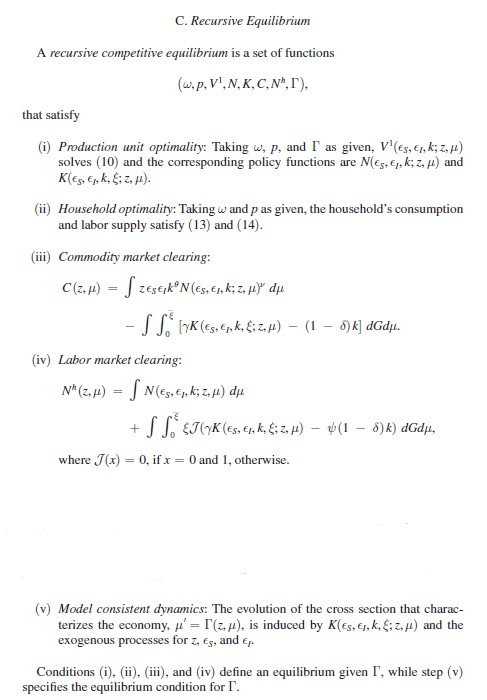
\includegraphics[width=0.35\textwidth]{Figures/bachman_et_al_equilibrium_definition_snip.jpg}}
\caption[Equilibrium in Bachmann \textit{et al} (2013)]{\label{fig:bachman_et_al_equilibrium_definition_snip} Equilibrium definition in Bachmann \textit{et al} (2013)}
\end{figure}

\hyperlink{curveshift}{\beamerbutton{Back}}


\end{frame}